% !TeX program = latexmk
% !TeX root = dp_puzzle.tex
% English master manuscript. Edit this file directly after the initial assembly.
% Chinese review counterpart: main.tex and sections/*.tex.
% All chapters and table bodies are inline; figures and bibliography are shared.
\RequirePackage[T1]{fontenc}
\documentclass[conference,10pt,letterpaper]{IEEEtran}
\usepackage[no-math]{fontspec}
\setmainfont{TeX Gyre Termes}
\setsansfont{TeX Gyre Heros}
\setmonofont{TeX Gyre Cursor}
\usepackage{amsmath,amssymb}
\usepackage{graphicx}
\usepackage[caption=false,font=footnotesize]{subfig}
\usepackage{booktabs}
\usepackage{cite}
\usepackage[hidelinks]{hyperref}
\graphicspath{{figures/}}
\newcommand{\PaperTitle}{DP-Puzzle: Exploring Throughput Ratios in Multi-Precision Floating-Point Tensor Cores with Composable Dot-Product Units}
\title{\PaperTitle}
\author{\IEEEauthorblockN{Anonymous Submission}}
\hypersetup{pdfauthor={},pdftitle={\PaperTitle},pdfsubject={English manuscript}}
\newcounter{DACreferencepage}
\AtEndDocument{%
  \ifnum\value{page}>\value{DACreferencepage}\relax
    \PackageWarningNoLine{DAC2027}{References exceed one page}%
  \fi}
\begin{document}
\bstctlcite{DPBSTcontrol}
\maketitle

% BEGIN REVIEW PAIR: 00_abstract.tex
\begin{abstract}
Multi-precision tensor hardware must balance high- and low-precision throughput within a limited area budget. The same ratio can be realized by extending the reduction dimension K or by adding independent outputs along N, with different circuit and data-supply costs. DP-Puzzle shares arithmetic across a lane--group--DP hierarchy and uses specialized E and QE components to construct $1:2:6$, $1:2:8$, and $1:4:8$ ratios. Synthesis and activity-based power analysis of six DPs at 12\,nm and 1\,GHz show that K expansion reduces component area by 0.65\%--2.40\% and estimated low-precision active power by 2.02\%--3.97\% relative to N composition at matched peak throughput. Bandwidth analysis separates input reuse from accumulator capacity and output-port demand. Under a fixed core-area budget, all four K ratios occupy distinct latency- and energy-optimal regions of the H/Q/E workload space. Prefill workloads derived from three DeepSeek models favor $1:4:8$ under the reference W4A8 mapping, whereas FP4 experts and long contexts can shift some workloads toward $1:2:8$. These results connect dot-product circuit costs to mixed-precision compute demand for workload-driven ratio selection.
\end{abstract}
\begin{IEEEkeywords}
Composable Dot-Product Architecture, Multi-Precision Tensor Cores, Throughput Ratios, Hardware Cost--Performance Trade-offs
\end{IEEEkeywords}
% END REVIEW PAIR: 00_abstract.tex

% BEGIN REVIEW PAIR: 01_introduction.tex
\section{Introduction}
\label{sec:introduction}
Low-precision floating-point computation is changing the demands that AI models place on tensor hardware. DeepSeek-V3 uses FP8 for forward and backward matrix multiplications in its main linear layers~\cite{deepseekv3}. GLM-4.5 uses online FP8 quantization to accelerate rollout inference during reinforcement learning while retaining BF16 parameter updates~\cite{glm45}. DeepSeek-V4 further quantizes MoE expert weights to MXFP4 and uses MXFP4 activations and dot products in its long-context attention indexer~\cite{deepseekv4}. Low-bit storage, however, does not always imply low-bit multiplication, and sensitive operations still require higher precision. Hardware must therefore support multiple execution precisions and allocate their throughput within area and power limits. We denote 16-, 8-, and 4-bit floating-point computation by H, Q, and E, respectively, and study their peak throughput ratios.

Commercial throughput ratios are becoming more diverse. Normalized to each chip's dense 16-bit matrix peak, NVIDIA B200, AMD MI355X, and Huawei Ascend 950PR use the conventional $1:2:4$ ratio~\cite{nvidiahgx,amdmi355x,huawei950}. NVIDIA B300 adopts $1:2:6$~\cite{nvidiahgx}, AMD MI455X provides approximately $1:4:8$~\cite{amdmi455x}, and Huawei's published Ascend 960PR development roadmap targets $1:2:8$~\cite{huawei960roadmap}. Provisioning additional low-precision capacity is a forward-looking architectural decision: chip design, verification, fabrication, and deployment take longer than model and quantization development. Precision demand observed during architecture design may therefore differ from demand during deployment. Ratio selection must anticipate this evolution when allocating resources.

Published specifications reveal the selected ratios but do not establish how they are implemented or how much usable throughput their additional area, power, and bandwidth deliver. Even at the same ratio, reduction length, output parallelism, and backend sharing change both resource costs and the data supply needed to sustain peak throughput. Prior work studies datapath reuse, numerical formats, and hardware costs~\cite{transdot2026,paretomac2025,zhao2026mxlike}, but reproducible comparisons of throughput ratios and their implementation alternatives remain limited. A common framework is needed to relate ratios, circuit organization, and resource constraints to workloads with different precision demands.

We present DP-Puzzle, which combines a shared multi-precision dot-product unit with specialized E and QE components for incremental low-precision capacity. Expansion along the reduction dimension $K$ connects these components to a common alignment and fused-output backend. Composition along the output dimension $N$ uses complete DPs to produce independent outputs. We first compare these organizations at matched absolute peak throughput for each precision, then deploy the K-expanded designs under the same total core-area budget. H/Q/E workload fractions determine the boundaries between latency- and compute-energy-optimal choices, linking unit costs, deployable core counts, and execution precision.

The contributions are:

\begin{enumerate}
  \item \textbf{A shared multi-precision dot-product microarchitecture.} Compact decoding, segmented multiplication, group alignment, and a common partial-sum representation share arithmetic across lanes, groups, and DPs, supporting BF16/FP16, MXFP8/6/4, NVFP4, HiF4, and their scale processing.
  \item \textbf{Low-precision specialization and two expansion methods.} E and QE frontends remove resources for unsupported precisions. K expansion shares the backend, whereas N composition provides independent outputs. Six DPs characterized under identical conditions quantify component costs, complemented by an analysis of input bandwidth and accumulator storage.
  \item \textbf{An area-constrained workload model.} Integer core deployment, mode throughput, and active power determine compute time and energy across four ratios. Prefill trajectories derived from fixed DeepSeek model structures show how context length and expert execution precision affect ratio selection.
\end{enumerate}

Section~\ref{sec:background} presents the background and motivation. Sections~\ref{sec:architecture} and~\ref{sec:expansion} describe the baseline DP and its specialization and composition. Section~\ref{sec:evaluation} evaluates circuit costs and bandwidth trade-offs. Section~\ref{sec:workload} analyzes workloads under an area constraint, and Section~\ref{sec:conclusion} concludes.
% END REVIEW PAIR: 01_introduction.tex

% BEGIN REVIEW PAIR: 02_background.tex
\section{Background and Motivation}
\label{sec:background}

\subsection{Floating-Point and Microscaling Formats}
\label{sec:formats}

We write fixed-point formats as $\mathrm{S}x\mathrm{P}y$ or $\mathrm{U}x\mathrm{P}y$, where $x$ counts integer bits excluding the sign and $y$ counts fractional bits. The signed form has one additional sign bit and width $1+x+y$; the unsigned form has width $x+y$. This notation specifies widths rather than two's-complement or sign--magnitude encoding. The precision-family label I refers exclusively to INT8.

A floating-point tensor's representation depends on both its element encoding and any shared block scale, as shown in Fig.~\ref{fig:fpformats}. BF16 and FP16 do not require an additional block scale; their exponent and significand widths determine dynamic range and precision~\cite{burgess2019bfloat16,ocpmx2023}. Microscaling formats combine low-bit elements, such as E5M2, E4M3, E3M2, E2M3, E2M1, or S1P2, with a shared scale. For block size $g$, OCP MXFP8/6/4 use $g=32$ and an E8M0 scale~\cite{ocpmx2023}; NVFP4 uses local blocks of $g=16$, E2M1 elements, and an E4M3 scale~\cite{nvidia2024nvfp4}. HiF4 uses $g=64$, S1P2 elements, an unsigned E6M2 base scale, and one-bit micro-exponents shared by every 8 and 4 elements~\cite{hifloat4}. Element encoding determines decoding and multiplication, block size determines reduction boundaries, and scale encoding determines how group results are scaled.

\begin{figure}[t]
\centering
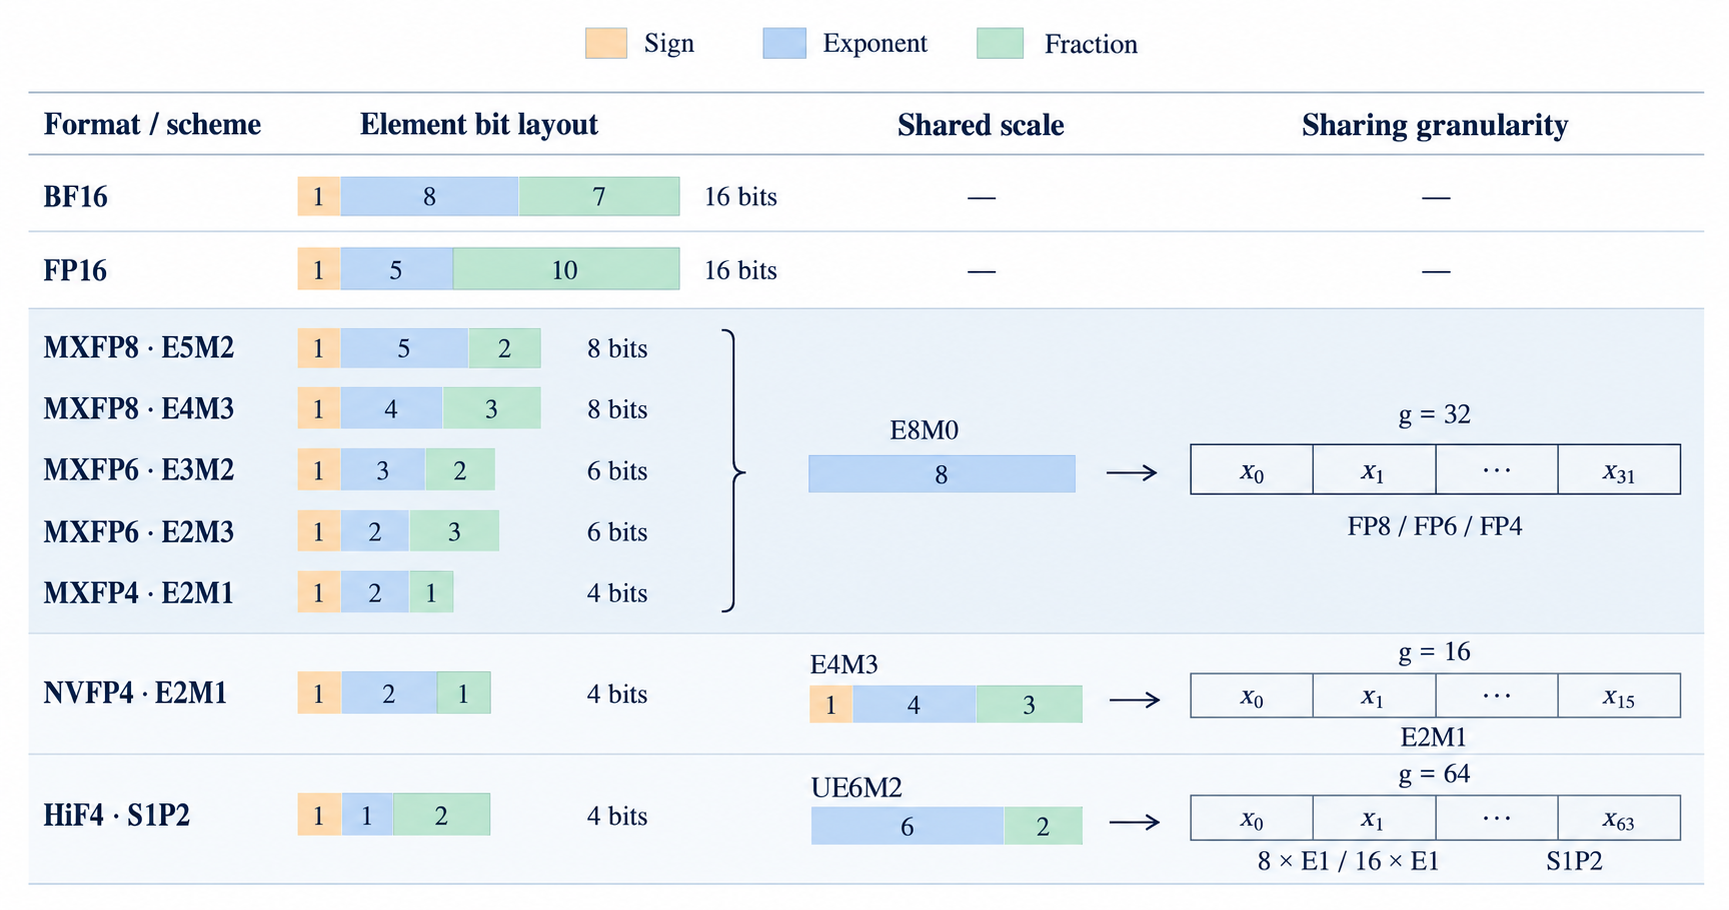
\includegraphics[width=\columnwidth]{fp_format.png}
\caption{Element encodings and shared scales~\cite{ocpmx2023,nvidia2024nvfp4,hifloat4}. Field labels denote bit widths; $g$ is the group size.}
\label{fig:fpformats}
\end{figure}


\subsection{Tensor Computation and Dot-Product Units}
\label{sec:tensor_organization}

For matrix multiplication and accumulation $D=C+AB$, $M$ and $N$ are output dimensions and $K$ is the reduction dimension. A tensor-array processing element (PE) may use separate multipliers and adders, fused multiply-add (FMA), or local dot products. These choices affect power, performance, and area (PPA). Separate operations permit independent scheduling but normalize and round intermediate floating-point results. FMA combines one multiplication and addition with a single final rounding. A dot-product unit aligns and reduces multiple products before shared accumulation and output processing, amortizing these costs across the inner product~\cite{lutzFusedFP84Way2024}.

We use a local DP as the array building block, with a baseline native FP16/BF16 reduction length of $K=16$. This granularity agrees with the dot-product accumulation granularity identified for Hopper and Blackwell in prior numerical modeling work~\cite{xie2025mmasim}. Each mode and ratio has its own native reduction length. Longer GEMMs connect partial sums across multiple DP requests. A DP accepts explicit C and produces D; accumulation state across requests resides outside the unit. Our bandwidth analysis assumes row/column broadcast and output residency, with storage location, interleaved contexts, and port requirements treated as model parameters rather than an implemented array memory system.

Formats with and without shared scales fit a common local dot-product structure. Following the OCP dot-product definition, a shared scale can be factored out of the reduction~\cite{ocpmx2023}. Partition $L$ products into $G=\lceil L/g\rceil$ scale groups, zero-pad the final group if necessary, and include an addend $c$:
\begin{equation}
d=c+\sum_{j=0}^{G-1}X_j^{(A)}X_j^{(B)}
\underbrace{\sum_{i=0}^{g-1}P_{j,i}^{(A)}P_{j,i}^{(B)}}_{q_j}.
\label{eq:blockdot}
\end{equation}
Here, $X_j^{(A)}$ and $X_j^{(B)}$ are the two operand scales for group $j$, $P_{j,i}^{(A)}$ and $P_{j,i}^{(B)}$ are decoded elements, and $q_j$ is the group dot product. HiF4 micro-exponents are included in element decoding. Setting $X_j^{(A)}=X_j^{(B)}=1$ gives ordinary dot-product accumulation for unscaled formats.

Equation~\eqref{eq:blockdot} exposes common boundaries for element multiplication and alignment, local reduction, scale processing, and accumulation across groups. These boundaries support arithmetic reuse and hierarchical composition. The equation specifies the computation; internal widths, operation ordering, and rounding positions remain implementation choices~\cite{ocpmx2023}.



\subsection{Datapath Reuse and Design-Space Exploration}
\label{sec:datapath_sharing}

Multi-precision units share multiplication, alignment, and reduction hardware to reduce the costs of separate datapaths. TransDot reconfigures multipliers and shifters across precisions, sharing resources between wide operations and parallel low-precision dot products~\cite{transdot2026}. MPICC decodes different formats into a common internal representation~\cite{huangMPICCMultiplePrecisionInterCombined2025}. Fused FP8 dot-product work compares dedicated backends with reuse of an FP32 FMA adder, highlighting accumulation, normalization, and rounding as additional sharing opportunities~\cite{lutzFusedFP84Way2024}.

Design-space exploration also connects numerical formats to hardware costs. Crafton et al. jointly explore low-precision formats and MAC microarchitectures using numerical-error, area, and power Pareto trade-offs~\cite{paretomac2025}. MX-like Tensor Core evaluates shared scales together with weight and activation formats~\cite{zhao2026mxlike}. At the array level, Timeloop explores mappings and organizations through loop tiling, spatial unrolling, and memory hierarchies, including tiling along $K$~\cite{timeloop2019}. These studies primarily optimize unit structures, formats, or array parameters. They provide limited direct comparison of 16-/8-/4-bit peak throughput ratios as independent design variables and of alternative implementations of the same ratio.



\subsection{Motivation for Throughput-Ratio Exploration}
\label{sec:commercial_ratios}
\label{sec:ratio_motivation}

Table~\ref{tab:vendor_ratios} summarizes representative products and development roadmaps. Normalized to each product's 16-bit matrix peak, ratios extend from $1:2:4$ to $1:2:6$, approximately $1:4:8$, and a roadmap target of $1:2:8$. This diversity makes low-precision provisioning an explicit architectural choice. Given the different development timescales of chips and models, provisioning must address both current workloads and future low-precision demand.

\begin{table}[t]
\centering
\caption{Per-device matrix peaks (PFLOP/s) and roadmap target.}
\label{tab:vendor_ratios}
\begingroup\footnotesize\setlength{\tabcolsep}{3pt}
\begin{tabular*}{\columnwidth}{@{\extracolsep{\fill}}lrrrl@{}}\toprule
Product & 16-bit & 8-bit & 4-bit & Ratio \\\midrule
B200 SXM~\cite{nvidiahgx} & 2.250 & 4.500 & 9.000 & $1:2:4$ \\
MI355X~\cite{amdmi355x} & 2.517 & 5.033 & 10.066 & $1:2:4$ \\
Ascend 950PR~\cite{huawei950} & 0.432 & 0.865 & 1.730 & $1:2:4$ \\
\midrule
B300 SXM~\cite{nvidiahgx} & 2.250 & 4.500 & 13.500 & $1:2:6$ \\
\midrule
Rubin GPU~\cite{nvidiaverarubin} & 4.000 & 17.500 & 35.000 & $\approx 1:4:8$ \\
MI455X~\cite{amdmi455x} & 5.033 & 20.133 & 40.265 & $1:4:8$ \\
\midrule
Ascend 960PR$^\dagger$~\cite{huawei960roadmap} & 1.000 & 2.000 & 8.000 & $1:2:8$ \\
\bottomrule
\end{tabular*}
\par\smallskip
\parbox{\columnwidth}{\raggedright Product rows use dense matrix peaks; $\dagger$ R\&D roadmap target.}
\endgroup
\end{table}

Two questions follow. First, how can shared arithmetic, specialized low-precision components, and DP composition realize a target ratio? Second, at matched absolute peak throughput for every precision, how do internal expansion along $K$ and array-level expansion along $M/N$ differ in area, power, bandwidth, and usable throughput? K expansion increases reduction parallelism for one output, whereas M/N expansion increases independent outputs, changing backend sharing and data-supply requirements. A composable DP and a common PPA and bandwidth model make these alternatives concrete and comparable. Section~\ref{sec:architecture} establishes the shared baseline; Section~\ref{sec:expansion} describes specialization and the two composition methods.
% END REVIEW PAIR: 02_background.tex

% BEGIN REVIEW PAIR: 03_architecture.tex
\section{Shared Multi-Precision Dot-Product Microarchitecture}
\label{sec:architecture}

DP-Puzzle shares arithmetic through a lane--group--DP hierarchy (Fig.~\ref{fig:dp_architecture}). Lanes map formats onto common multiplication and local alignment paths; groups apply block scales and produce a uniform partial-sum representation; the DP shares global alignment and fused accumulation. This boundary localizes NVFP4/HiF4 scale processing within each group and provides a common interface for specialized low-precision frontends. All modes use an eight-stage pipeline that accepts one independent request per cycle.

\subsection{Organization and Width Parameters}
\label{sec:brick_definition}
Table~\ref{tab:precision_families} defines the precision families. A suffix gives the number of element pairs processed per cycle. Each T1H2I4Q4E8 lane covers the eight elements sharing a HiF4 second-level micro-exponent. Two lanes form a group covering an NVFP4 block of 16 elements. Larger blocks broadcast a common scale to multiple groups without changing quantization granularity. Four groups form the T8H16I32Q32E64 baseline, whose modes use the shared resources mutually exclusively.
\begin{table}[t]
\centering
\caption{Precision families and supported numerical formats.}
\label{tab:precision_families}
\small
\setlength{\tabcolsep}{4pt}
\begin{tabular}{cl}
\toprule
Abbreviation & Numerical formats \\
\midrule
T & TF32 \\
H & FP16, BF16 \\
Q & MXFP8 (E4M3, E5M2), MXFP6 (E2M3, E3M2) \\
E & MXFP4, NVFP4, HiF4 \\
I & INT8 \\
\bottomrule
\end{tabular}
\end{table}

Table~\ref{tab:datapath_parameters} defines widths in bits. The signals $\mathrm{sop}$, $\mathrm{scale\_mant}$, and $\mathrm{anchor}$ denote the partial-sum magnitude, the product of the two scale significands, and the exponent coordinate. Let $\ell(n)=\lceil\log_2 n\rceil$. The counts $n_{\mathrm{tree}}$, $n_{\mathrm{lane}}$, and $n_{\mathrm{group}}$ denote reduction-tree leaves per lane, lanes per group, and groups per DP; the baseline uses 4, 2, and 4. The formulas express width relationships, while the numerical settings identify the baseline configuration.
\begin{table}[t]
\centering
\caption{Datapath width parameters and their derivation. Signed sums include the sign bit; magnitude widths exclude it.}
\label{tab:datapath_parameters}
\footnotesize
\setlength{\tabcolsep}{3pt}
\begin{tabular}{lll}
\toprule
Parameter & Meaning & Definition / setting \\
\midrule
$\mathrm{Lane}_{\mathrm{align}}$ & Unsigned local window & $28$ \\
$\mathrm{Lane}_{\mathrm{sop}}$ & Signed lane sum & $\mathrm{Lane}_{\mathrm{align}}+1+\ell(n_{\mathrm{tree}})$ \\
$\mathrm{Group}_{\mathrm{mag}}$ & Group magnitude & $\mathrm{Lane}_{\mathrm{sop}}+\ell(n_{\mathrm{lane}})-1$ \\
$\mathrm{Group}_{\mathrm{frac}}$ & Group fractional bits & Format dependent \\
$\mathrm{Scale}_{\mathrm{in}}$ & One scale significand & $4$ \\
$\mathrm{Scale}_{\mathrm{sop}}$ & Compact group magnitude & $14$ \\
$\mathrm{Scale}_{\mathrm{mant}}$ & Scale product & $2\,\mathrm{Scale}_{\mathrm{in}}$ \\
$\mathrm{DP}_{\mathrm{align}}$ & Unsigned global window & $39$ \\
$\mathrm{DP}_{\mathrm{sop}}$ & Signed accumulated sum & $\mathrm{DP}_{\mathrm{align}}+1+\ell(n_{\mathrm{group}}+1)$ \\
\bottomrule
\end{tabular}
\end{table}

\begin{figure}[t]
\centering
\includegraphics[width=\columnwidth]{baseline_arch.png}
\caption{Hierarchical lane--group--DP architecture. Lanes share multipliers and local shifters; groups apply scale significands and recompute anchors; the DP shares global alignment and accumulation, with an integer bypass around floating-point alignment and output processing.}
\label{fig:dp_architecture}
\end{figure}

\subsection{Lane: Decoding for Multiplier and Shifter Reuse}
\label{sec:unpack_recode}
\label{sec:full_brick}

\textbf{Common decoding.} Figure~\ref{fig:data_unpack} maps packed inputs to exponent, significand, and sign fields. Each operand side of a lane has two H1/Q2/E4 field groups; TF32 occupies the entire lane. Together, the groups provide 20 exponent bits, 32 significand bits, and 8 sign bits. T/H decoding restores the significand and hidden bit, Q uses an internal E5M3 representation, and INT8 separates sign and magnitude. MXFP4/NVFP4 absorb the E2M1 element exponent into a four-bit U3P1 magnitude. HiF4 incorporates its first-level micro-exponent into an U2P2 magnitude while retaining the lane-shared second-level micro-exponent. E thus enters a fixed-point product path without per-element floating-point alignment. Special-value flags propagate separately.
\begin{figure}[t]
\centering
% Author figure update: whole-lane counts should read 2x FP16 and 8x E.
% The 10/16/4-bit fields describe one field group; each lane contains two.
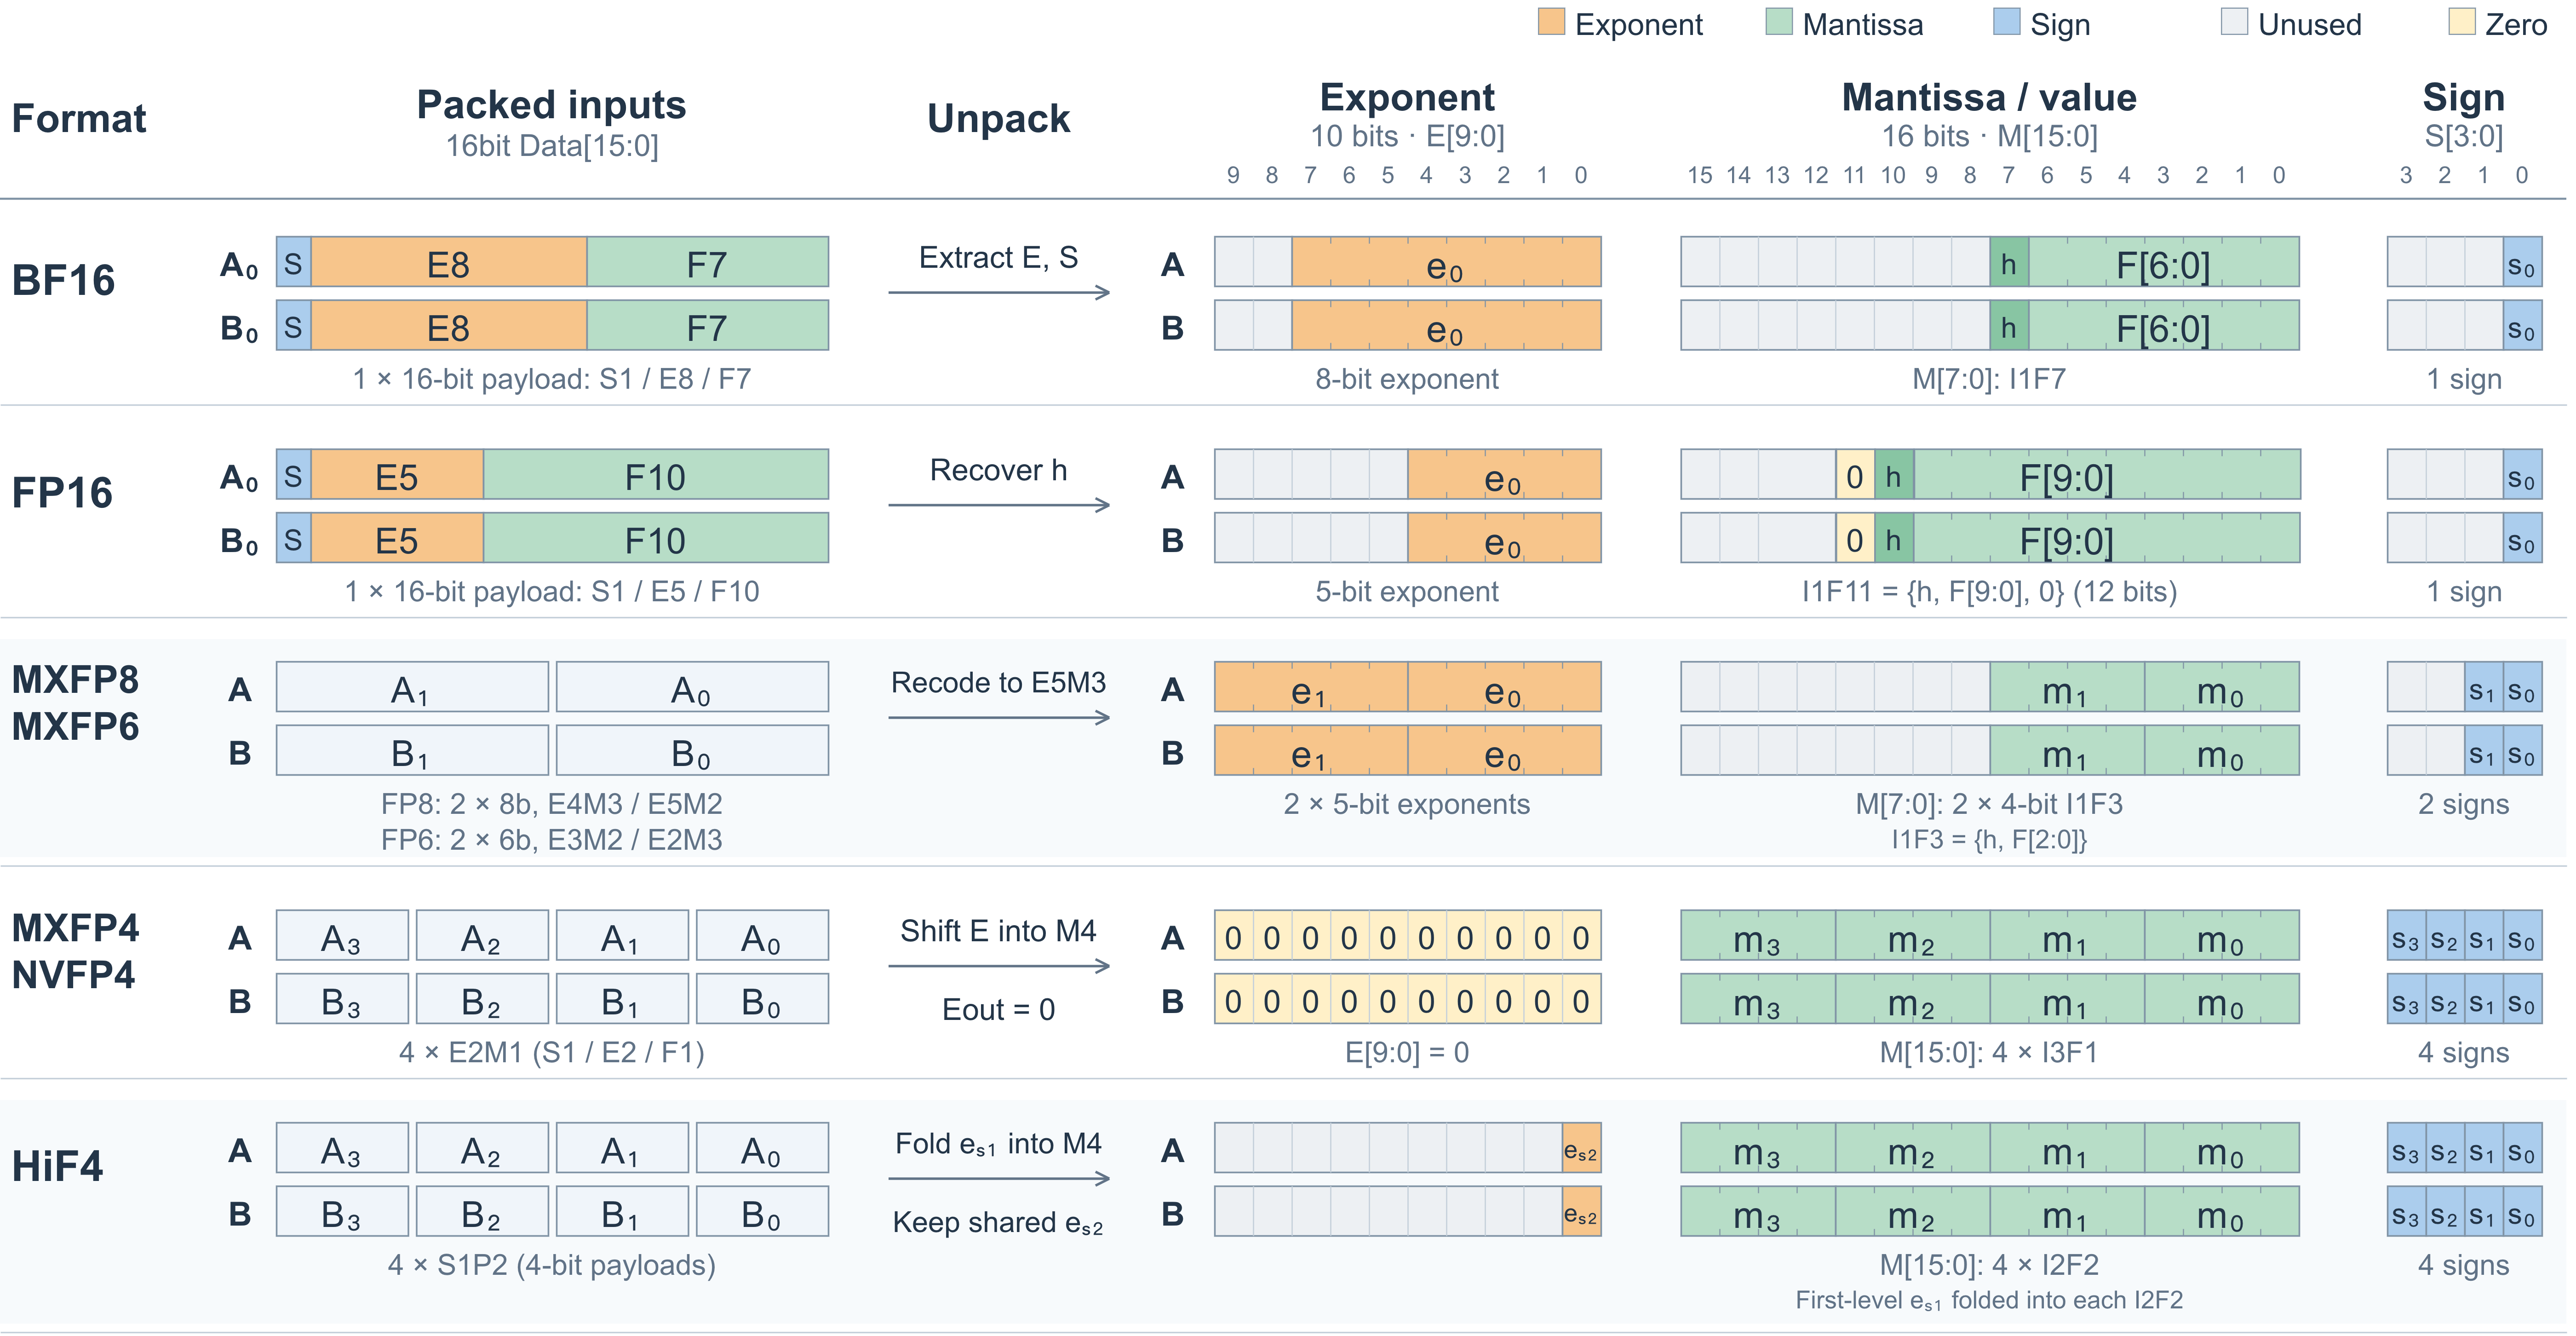
\includegraphics[width=\columnwidth]{unpack_layout.png}
\caption{Operand unpacking for shared arithmetic. T/H retain exponent and significand fields; Q uses a common internal E5M3 representation; INT8 uses sign and magnitude. E formats absorb element exponents into fixed-point magnitudes, while HiF4 retains its lane-shared micro-exponent. Unused field bits are zero-filled.}
\label{fig:data_unpack}
\end{figure}

\textbf{Segmented multiplier reuse.} Ten-Four shares multipliers among classes of significand widths~\cite{rout2026tenfourv2}. We combine segmented products for higher precision and route independent elements for low-precision parallelism. Each lane contains two banks of $8\times8$, $8\times4$, $4\times8$, and $4\times4$ multipliers. TF32/FP16 combine partial products; BF16 uses the wide multiplier directly; Q/E map independent elements to narrow inputs; and INT8 reuses the wide product and cross-product reconstruction paths. Input selection and product composition handle format differences without a separate complete multiplier array for every format.

\textbf{Common-width shifter reuse.} T/H/Q products are statically zero-padded according to their binary-point positions into a common $\mathrm{Lane}_{\mathrm{align}}$-bit magnitude window. They align to $\mathrm{anchor}_{\mathrm{lane}}$, the maximum effective element-exponent sum across both lanes before bias removal. Four 28-bit right shifters therefore serve all local T/H/Q alignment, with 1, 2, and 4 active paths, respectively. E/INT8 bypass this network. E first forms pairwise sums and then enters the shared reduction tree; HiF4 applies its small second-level micro-exponent shift to the lane sum. All modes produce a $\mathrm{Lane}_{\mathrm{sop}}$-bit partial sum.

\subsection{Group: Scale Fusion and Anchor Recompute}

\textbf{Compact scale multiplication.} NVFP4/HiF4 scales include significands, so exponent addition alone cannot implement scaling. Because both lanes share a scale, the group reduces their sums and extracts the magnitude before applying $\mathrm{scale\_mant}$. Removing structural low-order zeros allows both formats to share an unsigned $\mathrm{Scale}_{\mathrm{sop}}\times\mathrm{Scale}_{\mathrm{mant}}$ multiplier instead of replicating scale multiplication per element. In the baseline, the group magnitude is U14 and the product of two U4 scale significands is U8. A U14$\times$U8 multiplication retains its full result, which is padded with low-order zeros to form the $\mathrm{Group}_{\mathrm{mag}}$-bit $\mathrm{sop}$. MX power-of-two scales modify only the exponent and bypass this multiplication. Table~\ref{tab:group_formats} gives the fixed-point positions at the lane and group outputs.

\begin{table}[t]
\centering
\caption{Lane and group fixed-point formats for the baseline configuration. SxPy specifies one sign bit, x integer bits, and y fractional bits. Group outputs keep sign and magnitude separate; y gives $\mathrm{Group}_{\mathrm{frac}}$.}
\label{tab:group_formats}
\small
\setlength{\tabcolsep}{4pt}
\begin{tabular}{lccc}
\toprule
Format & Lane & Group & $\mathrm{bias}$ \\
\midrule
TF32       & S2P28  & S3P28  & 127 \\
FP16       & S3P27  & S4P27  & 15  \\
BF16       & S3P27  & S4P27  & 127 \\
Q          & S4P26  & S5P26  & 15  \\
MXFP4      & S9P21  & S10P21 & 0   \\
NVFP4/HiF4 & S9P21  & S12P19 & 0   \\
INT8       & S17P13 & S18P13 & --- \\
\bottomrule
\end{tabular}
\end{table}

\textbf{Anchor Recompute.} To share the backend across different binary-point positions, each group uses $\mathrm{anchor}$ as the exponent associated with the magnitude's most significant physical bit. A finite floating-point group result satisfies
\begin{equation}
\mathrm{value}=(-1)^{\mathrm{sign}}\mathrm{sop}\,
2^{\mathrm{anchor}-(\mathrm{Group}_{\mathrm{mag}}-1)}.
\label{eq:group_value}
\end{equation}
Let $\mathrm{scale\_exp}$ be the sum of the two unbiased scale exponents and $\mathrm{bias}$ the element-exponent bias. Then
\begin{equation}
\begin{aligned}
\mathrm{offset}&=\mathrm{Group}_{\mathrm{mag}}-1-\mathrm{Group}_{\mathrm{frac}}
                 -2\,\mathrm{bias},\\
\mathrm{anchor}&=\mathrm{anchor}_{\mathrm{lane}}+\mathrm{scale\_exp}+\mathrm{offset}.
\end{aligned}
\label{eq:anchor_recompute}
\end{equation}
The format-dependent $\mathrm{offset}$ combines binary-point and element-bias corrections, allowing anchor computation to proceed in parallel with significand reduction. E formats already incorporate element exponents into their magnitudes, so both $\mathrm{anchor}_{\mathrm{lane}}$ and $\mathrm{bias}$ are zero. Unscaled formats use zero $\mathrm{scale\_exp}$. This representation unifies the scaled NVFP4/HiF4 results with the bypassed results of other modes.

\textbf{Comparison exponent and bidirectional alignment.} Cancellation within a group can introduce leading zeros. Comparing raw anchors would then waste part of the global alignment window. The group computes
\begin{equation}
\begin{aligned}
\mathrm{lzc}&=\operatorname{clz}_{\mathrm{Group}_{\mathrm{mag}}}(\mathrm{sop}),\\
\mathrm{anchor}_{\mathrm{nz}}&=\mathrm{anchor}-\mathrm{lzc}.
\end{aligned}
\label{eq:anchor_nonzero}
\end{equation}
For a nonzero magnitude, the leading-zero count is at most $\mathrm{Group}_{\mathrm{mag}}-1$. A zero magnitude has count $\mathrm{Group}_{\mathrm{mag}}$ and is excluded from exponent comparison. The leading-bit exponent $\mathrm{anchor}_{\mathrm{nz}}$ selects the global $\mathrm{anchor}_{\max}$, while the raw anchor determines the net shift:
\begin{equation}
\begin{aligned}
\mathrm{shift}&=\mathrm{lzc}-(\mathrm{anchor}_{\max}-\mathrm{anchor}_{\mathrm{nz}})\\
             &=\mathrm{anchor}-\mathrm{anchor}_{\max}.
\end{aligned}
\label{eq:group_shift}
\end{equation}
Positive, negative, and zero shifts select left shift, right shift, and passthrough, respectively. One bidirectional shift therefore combines normalization and alignment. The group generates the magnitude and both anchors; the physical shift takes place in the DP's global window.

\subsection{DP: Fused Accumulation and Integer Bypass}

The DP connects group results and $C$ to a common global alignment and accumulation path. Floating-point mode selects $\mathrm{anchor}_{\max}$ from finite nonzero group comparison exponents and the effective exponent of $C$. Group magnitudes are zero-padded to $\mathrm{DP}_{\mathrm{align}}$ bits, shifted according to~\eqref{eq:group_shift}, and restored to $\mathrm{DP}_{\mathrm{align}}+1$-bit signed values. A subnormal $C$ retains its unnormalized significand; its effective exponent provides an upper bound for comparison, avoiding a separate leading-zero detector.

The baseline compresses four groups with a 4:2 compressor, incorporates $C$ with a 3:2 compressor, and uses a single carry-propagate adder to produce the $\mathrm{DP}_{\mathrm{sop}}$-bit sum. INT8 mode statically places group results and the INT32 addend in a common integer coordinate, bypassing floating-point exponent comparison and bidirectional alignment while reusing the accumulator. The output bypasses floating-point normalization and rounding, extracts INT32, and wraps on integer overflow.

Floating-point output uses round-to-nearest, ties-to-even. Local and global magnitude right shifts truncate toward zero; local fixed-point E reduction introduces no truncation. Precision enables follow each request and suppress unused register updates and input activity, allowing formats to change on successive cycles.
% END REVIEW PAIR: 03_architecture.tex

% BEGIN REVIEW PAIR: 04_expansion.tex
\section{Low-Precision Specialization and Throughput-Ratio Expansion}
\label{sec:expansion}

The baseline provides $16/32/64$ H/Q/E MACs per cycle, corresponding to $1:2:4$. Additional low-precision capacity can extend the reduction length $K$ within a DP or add independent output columns $N$. K expansion shares the output backend; N expansion increases output parallelism. Both require inexpensive low-precision components, but differ in where partial results merge and whether accumulation and rounding remain independent.

Figure~\ref{fig:kn_datapaths} compares the two organizations at a common group boundary. K expansion merges partial sums before producing a final floating-point result. N expansion gives the added components complete backends and independent outputs.

\begin{figure}[t]
\centering
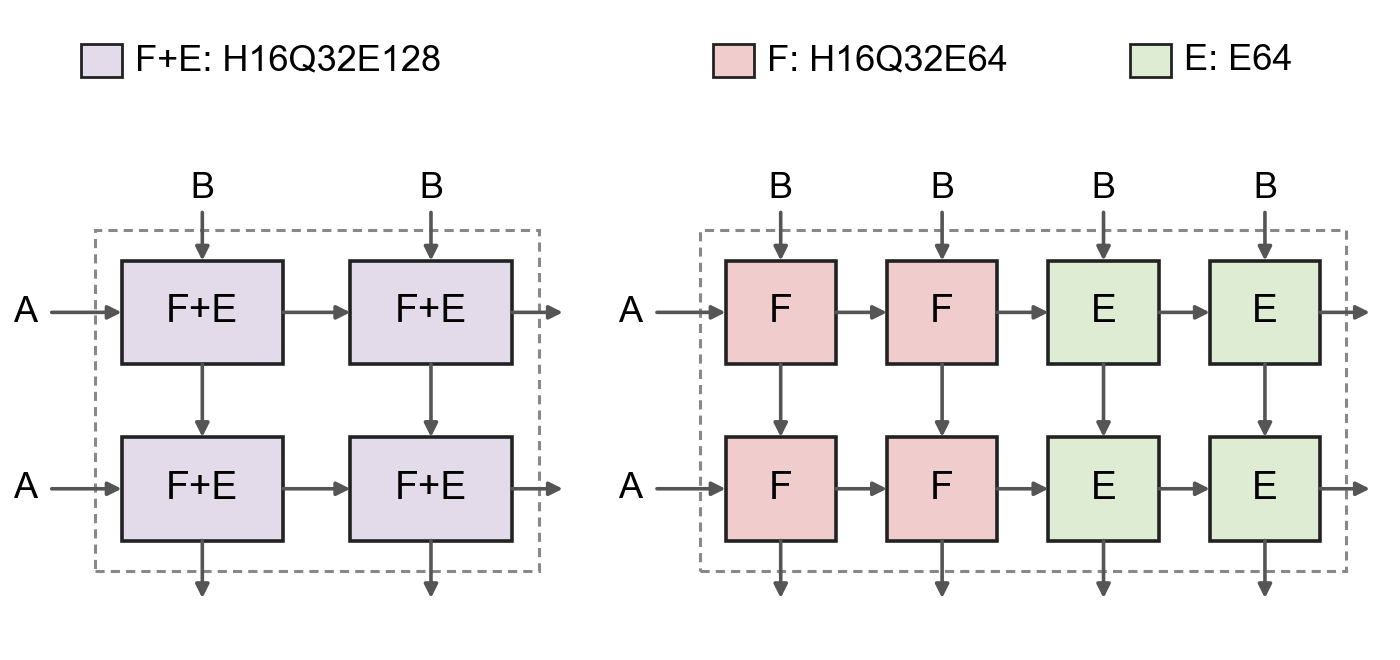
\includegraphics[width=\columnwidth]{kn_composition.png}
\caption{Internal K expansion versus independent N outputs. Dashed outlines mark complete DPs; arrows show arithmetic flow, not array scheduling. Exact capacity-matched compositions are listed in Table~\ref{tab:brick_compositions}.}
\label{fig:kn_datapaths}
\end{figure}

\subsection{Specialized E and QE Components}
\label{sec:specialized_midgroups}

\textbf{E specialization narrows arithmetic and storage.} The shared baseline retains wide multiplier leaves, reduction hardware, and format selection even when executing E. A specialized E lane uses eight $4\times4$ multipliers and removes high-precision product reconstruction, element-exponent comparison, and wide local alignment. Pairwise addition immediately follows multiplication, retaining four 10-bit pairs. A balanced tree produces a 12-bit sum, which is extended to 14 bits before incorporating the HiF4 second-level micro-exponent. MXFP4/NVFP4 use fixed zero padding at the same point. Keeping this small exponent adjustment within the narrow path avoids propagating its control through a wider network.

Two E lanes form an E16 group. Group addition and magnitude extraction occur before scale processing, leaving a 14-bit magnitude and an eight-bit scale coefficient at the scale stage. The product retains 22 bits; the MXFP4 bypass enters the same container through low-order zero padding. Leading-zero detection operates on this narrow container before low-order padding connects it to the common group interface. Such padding preserves the leading-zero count of a nonzero magnitude, so the specialized frontend maintains the shared backend's coordinates without restoring wide internal arithmetic.

\textbf{QE specialization retains Q alignment.} A QE lane removes T/H/INT8 paths and uses eight four-bit multipliers, four of which are active in Q mode. Q still requires five-bit element exponents, six-bit product exponents, and wide local alignment, so Q/E share a wider reduction tree. E bypasses alignment and incorporates its local micro-exponent after the tree. Two lanes form a Q8E16 group. Relative to E specialization, QE pays for Q alignment and wider registers in exchange for reuse between FP8/6 and FP4.

Both components output a sign, magnitude, exponent information, and special-value status. This common representation decouples the composition boundary from internal widths: a low-precision frontend can connect either to the baseline's shared backend or to an independent backend forming a complete DP.

\subsection{Internal Expansion Along K}
\label{sec:k_expansion}

K expansion assigns additional reduction segments of the same output to new groups. The four baseline multi-precision groups remain unchanged. Adding two E16, four E16, or four Q8E16 groups produces H16Q32E96, H16Q32E128, or H16Q64E128, respectively. Spatial parallelism increases low-precision products without changing high-precision capacity, pipeline depth, or the one-request-per-cycle initiation rate.

\textbf{Input and alignment paths grow with participating sources.} New groups receive additional A/B segments and scales, while the DP retains one $C$. All participating groups and $C$ select one global exponent, and each new source receives a global shifter and sign-restoration path. The baseline and extension may compute separate MAX candidates, but must merge them before alignment. Independently aligning and summing each branch before realigning their results would add serial operations and another truncation point.

\textbf{Additional products merge in carry-save form.} The two rows produced by compressing the baseline groups and $C$ feed the extension network directly. Two added groups combine with these rows through a 4:2 compressor. Four added groups first reduce to two rows, then merge with the baseline rows through another 4:2 compressor. A request selects either the baseline or extended row pair before the sole carry-propagate adder. This avoids serial carry propagation through separate extension and final sums. Seven input sources require a 43-bit result and nine require 44 bits; output normalization retains the corresponding growth bits.

\textbf{Participation masks control arithmetic and activity.} E extensions participate only in E mode, whereas QE extensions participate in Q/E modes. The mask follows each request and controls frontend updates, global MAX candidates, shifter inputs, and compressor leaves. Numerical zero and nonparticipation are distinct: participating special values must propagate, but stale special values in disabled groups must not affect the current result. The all-negative-zero condition also considers only participating terms. High-precision requests can therefore bypass extension compression while suppressing switching in unused frontends.

\subsection{Complete-DP Composition Along N}
\label{sec:n_expansion}

N expansion equips low-precision groups with independent global alignment, $C$ accumulation, and output processing, then places complete DPs alongside the baseline along output columns. Four E16 groups form E64, and four Q8E16 groups form Q32E64. Each DP computes a different output position: a row may share A, while each column receives its own B and $C$ and produces an independent D. Added columns do not participate in unsupported modes.

The standalone E64 uses a different local pipeline partition. Lanes retain narrow sums and micro-exponents; the group applies the micro-exponents and detects leading zeros in the full group magnitude. Its backend retains C leading-zero detection and a five-input adder tree. The internal E components instead use lane-local micro-exponent fusion, narrow magnitude detection, and the carry-save backend described above. Their format capacity and throughput match, but the circuits differ; the cost comparison includes these implementation differences.

Let $\mathcal F$, $\mathcal E$, and $\mathcal L$ denote complete baseline, E64, and Q32E64 DPs, and $\mathcal K_{126}$, $\mathcal K_{128}$, and $\mathcal K_{148}$ the three K-expanded DPs. Table~\ref{tab:brick_compositions} lists compositions with matched capacity. For $1:2:6$, two K-expanded DPs are compared with two baseline DPs plus one E64, matching absolute throughput with integer instances. Half an E64 is meaningful only for normalized cost accounting, not physical deployment.

\begin{table}[t]
\centering
\caption{Capacity-matched K/N compositions. Capacity is aggregate H/Q/E MACs per cycle.}
\label{tab:brick_compositions}
\begingroup\footnotesize\setlength{\tabcolsep}{3pt}
\begin{tabular*}{\columnwidth}{@{\extracolsep{\fill}}cllc@{}}\toprule
Ratio & K composition & N composition & Capacity \\\midrule
$1:2:4$ & $\mathcal F$ & $\mathcal F$ & 16/32/64 \\
$1:2:6$ & $2\mathcal K_{126}$ & $2\mathcal F+\mathcal E$ & 32/64/192 \\
$1:2:8$ & $\mathcal K_{128}$ & $\mathcal F+\mathcal E$ & 16/32/128 \\
$1:4:8$ & $\mathcal K_{148}$ & $\mathcal F+\mathcal L$ & 16/64/128 \\
\bottomrule
\end{tabular*}\endgroup
\end{table}

\subsection{Structural Trade-offs}
\label{sec:brick_composition}

K expansion increases input width per output, the number of globally aligned sources, and reduction fan-in while sharing $C$ handling, final addition, and rounding. N expansion retains shorter per-DP reductions and increases reuse of A across columns, but duplicates backends and maintains more live output partial sums. Equal peaks therefore need not imply equal input or accumulator requirements.

These differences also affect utilization. K expansion needs sufficiently long reductions; short-K tails may leave slots unused. N expansion needs enough independent outputs; narrow matrices may not fill the added columns. We next compare circuit costs at matched capacity, analyze bandwidth and accumulator state, and then evaluate the four K ratios under an explicit area model.
% END REVIEW PAIR: 04_expansion.tex

% BEGIN REVIEW PAIR: 05_evaluation.tex
\section{Hardware Implementation and Evaluation}
\label{sec:evaluation}

We first analyze baseline costs, then specialization and ratio expansion, and finally K/N composition at matched peak capacity. Circuit characterization supplies area and mode power to the workload model. Array bandwidth and accumulator storage are examined separately as structural constraints.

\subsection{Methodology}
\label{sec:eval_setup}

All six complete DPs are synthesized with Synopsys Design Compiler using a 12\,nm standard-cell library at TT, 0.7\,V, and 85$^\circ$C, targeting 1\,GHz with integrated clock gating. Each design retains eight pipeline stages and accepts one independent request per cycle. All satisfy post-synthesis setup, hold, and electrical constraints under these conditions. Area includes datapath logic, pipeline registers, and clock-gating cells, but excludes array storage and interconnect.

Power activity is driven by activations and weights from the first-layer MLP down-projection of Qwen3-8B~\cite{qwen3technicalreport}, mapped to BF16, MXFP8 E4M3, and MXFP4 E2M1. VCS gate-level simulation captures a stable 512-cycle window of continuous issue and generates SAIF activity for Power Compiler, which reports internal, net-switching, and leakage power~\cite{synopsysActivityPower}. Activity annotation covers all target objects, and RTL and gate-level numerical results agree. These are post-synthesis estimates before clock-tree synthesis and routing; routed parasitics and memory-access power are excluded.

We count one MAC as two FLOPs. In addition to total area and power, we report area efficiency $2K_f\nu/A$ and energy per FLOP $P_f/(2K_f\nu)$, where $K_f$ is the native product count in mode $f$ and $\nu$ is frequency. This separates total power growth from changes in the cost per operation.

\subsection{Baseline Area and Power Breakdown}
\label{sec:reuse_evaluation}
\label{sec:area_breakdown}

The baseline occupies 0.016165\,mm$^2$ and consumes 15.328, 16.002, and 11.197\,mW in BF16, MXFP8, and MXFP4 modes. Table~\ref{tab:baseline_breakdown} groups combinational logic and associated registers by function. Multiplication accounts for 24.15\% of area, whereas reduction and alignment together account for 38.91\%. Multiplier cost alone therefore does not explain the complete DP. Unpacking and exponent processing contribute another 27.21\%, reflecting format support, scaling, and coordinate handling.

\begin{table}[t]
\centering
\caption{Baseline functional shares (\%). H/Q/E use BF16/MXFP8/MXFP4. Power includes dynamic and leakage components.}
\label{tab:baseline_breakdown}
\begingroup\footnotesize\setlength{\tabcolsep}{3pt}
\begin{tabular*}{\columnwidth}{@{\extracolsep{\fill}}lrrrr@{}}\toprule
Function & Area & $P_H$ & $P_Q$ & $P_E$ \\\midrule
Multiplication & 24.15 & 15.87 & 14.55 & 16.07 \\
Reduction & 21.84 & 14.54 & 14.56 & 16.59 \\
Alignment & 17.07 & 20.51 & 20.74 & 13.31 \\
Exponent & 11.19 & 11.80 & 12.49 & 8.28 \\
Unpacking & 16.02 & 17.54 & 18.12 & 21.31 \\
Norm./round & 3.04 & 2.42 & 2.16 & 2.85 \\
Others & 6.70 & 17.32 & 17.39 & 21.59 \\
\bottomrule
\end{tabular*}\endgroup
\end{table}

Alignment accounts for 20.74\% of Q-mode power but 13.31\% in E mode, consistent with E bypassing element-exponent alignment. Unpacking and the remaining control, gating, and miscellaneous logic become relatively more prominent in E mode. Reducing element width does not proportionally reduce total DP power; low-precision specialization should also prune wide registers, exponent logic, and selection paths. These functional shares locate costs but do not attribute the entire difference between complete designs to a single optimization.

\subsection{Comparison with Existing Arithmetic Units}
\label{sec:related_dp_evaluation}

Table~\ref{tab:related_features} separates native input formats from datapath features. FPnew targets scalar and SIMD floating-point operations; Ten-Four combines multi-format dot products with integer accumulation; MPICC supports heterogeneous low-precision operands and stochastic rounding; MXDOTP focuses on native MXFP8 scaled dot products; and TransDot shares resources across multi-precision SIMD and dot-product operations. DP-Puzzle covers H/Q/E with block-scale processing and varies low-precision capacity through specialized frontends.

% BEGIN INLINE TABLE: tables/related_features.tex
% Entries refer to reported configurations, not hypothetical reconfiguration.
\begin{table*}[t]
\centering
\caption{Supported input formats and datapath features of related arithmetic units.}
\label{tab:related_features}
\begingroup\footnotesize\setlength{\tabcolsep}{3pt}
\def\Y{$\checkmark$}\def\N{$\times$}
\begin{tabular*}{\textwidth}{@{\extracolsep{\fill}}l*{14}{c}@{}}\toprule
& \multicolumn{9}{c}{Native input formats} & \multicolumn{5}{c}{Datapath features} \\
\cmidrule(lr){2-10}\cmidrule(lr){11-15}
Design & TF32 & FP16 & BF16 & FP8 & FP6 & FP4 & INT8 & INT4 & LOG4 & DP & MX & NVFP4 & HiF4 & SR \\\midrule
Ten-Four~\cite{rout2026tenfourv2} & \Y & \Y & \Y & \Y & \N & \N & \Y & \Y & \N & \Y & \Y & \N & \N & \N \\
MPICC~\cite{huangMPICCMultiplePrecisionInterCombined2025} & \N & \N & \N & \Y & \Y & \Y & \N & \Y & \Y & \Y & --- & \N & \N & \Y \\
MXDOTP~\cite{islamoglu2025mxdotp} & \N & \N & \N & \Y & \N & \N & \N & \N & \N & \Y & \Y & \N & \N & --- \\
FPnew~\cite{mach2020fpnew} & \N & \Y & \Y & \Y & \N & \N & \N & \N & \N & \N & \N & \N & \N & \N \\
TransDot~\cite{transdot2026} & \N & \Y & \N & \Y & \N & \Y & \N & \N & \N & \Y & \N & \N & \N & --- \\
\midrule
DP-Puzzle & \Y & \Y & \Y & \Y & \Y & \Y & \Y & \N & \N & \Y & \Y & \Y & \Y & \N \\
\bottomrule\end{tabular*}
\par\smallskip
\parbox{\textwidth}{\raggedright
$\checkmark$: supported; $\times$: absent from the reported configuration; ---: not established by the cited evidence.
DP: native multi-term dot product; MX/NVFP4/HiF4: integrated block-scale handling (MX indicates at least one MX format); SR: stochastic rounding.
FP8/FP4 denote element arithmetic and do not imply scale support. FPnew additionally supports FP32/64; TransDot supports FP32 FMA. MPICC supports heterogeneous operand combinations and FP12 emulation, which is not marked as native FP16.}
\endgroup
\end{table*}
% END INLINE TABLE: tables/related_features.tex
% BEGIN INLINE TABLE: tables/related_ppa.tex
% Sources and arithmetic conversions: references/notes/dp_comparison.md.
\begin{table*}[t]
\centering
\caption{Implementation conditions and precision-specific efficiency. Columns retain each work's reported technology and arithmetic boundary.}
\label{tab:related_dp}
\begingroup\footnotesize\setlength{\tabcolsep}{4pt}
\begin{tabular*}{\textwidth}{@{\extracolsep{\fill}}l*{6}{c}@{}}\toprule
Metric & Ten-Four~\cite{rout2026tenfourv2} & MPICC~\cite{huangMPICCMultiplePrecisionInterCombined2025} & MXDOTP~\cite{islamoglu2025mxdotp} & FPnew~\cite{mach2020fpnew} & TransDot~\cite{transdot2026} & This work \\\midrule
Structure & Fused DP & $n$-term MAC & Scaled DP & Vector FMA & FMA / DP & Scaled DP \\
Evaluation & Synthesis & Synthesis & Post-layout & Silicon & Post-layout & Synthesis \\
Technology (nm) & 7 (predictive) & 28 & 12 & 22FDX & 12 & 12 \\
Voltage (V) & 0.7 & 0.9 & 0.8 & 0.8 & 0.8 & 0.7 \\
Frequency (GHz) & 1.5$^a$ & 1.43 & 1.09 & 0.923 & 1.0 & 1.0 \\
Area ($\mu$m$^2$) & 1959.86 & 2295 & 3150 & 49\,000$^b$ & --- & 16\,165.12 \\
Accumulation & FP32/INT32 & FP12/INT8 & FP32 & Mode-specific & FP32$^c$ & FP32/INT32 \\
\midrule
\multicolumn{7}{l}{Energy efficiency (GFLOP/s/W)} \\
\quad FP16 & --- & --- & --- & 497.67 & 555.56 & --- \\
\quad BF16 & --- & --- & --- & 581.96 & --- & 2087.65 \\
\quad FP8 / MXFP8 & --- & 1948 & 2035 & 1244.78 & 1190.48 & 3999.50 \\
\quad FP4 / MXFP4 & --- & 5931 & --- & --- & 2439.02 & 11\,432.11 \\
\quad FP12 (emulated) & --- & 865.1 & --- & --- & --- & --- \\
\midrule
\multicolumn{7}{l}{Area efficiency (GFLOP/s/mm$^2$)} \\
\quad FP16 & --- & --- & --- & 151.43 & --- & --- \\
\quad BF16 & --- & --- & --- & 151.43 & --- & 1979.57 \\
\quad FP8 / MXFP8 & --- & 1246 & 5523.81 & 302.65 & --- & 3959.14 \\
\quad FP4 / MXFP4 & --- & 4985 & --- & --- & --- & 7918.28 \\
\quad FP12 (emulated) & --- & 415.4 & --- & --- & --- & --- \\
\bottomrule\end{tabular*}
\par\smallskip
\parbox{\textwidth}{\raggedright
---: unavailable here or inapplicable; it does not mean zero. One MAC/FMA is counted as two FLOPs; an $n$-term MAC is counted as $2n$ FLOPs.
$^a$Ten-Four targets 1.5 GHz and reports $F_{\max}=1.571$ GHz and total power 6.28 mW; no format-specific efficiency is inferred from that aggregate power.
$^b$FPnew area and nominal SIMD energy include the entire FPU; its FP8 encoding differs from MXFP8.
$^c$TransDot entries use dot products accumulated into FP32; energy efficiency is converted from reported pJ/FLOP.
MXDOTP and this work use MXFP8; this work's FP4 entries use MXFP4. FPnew/MXDOTP area efficiency is calculated from reported throughput and area. Different process nodes, accumulation formats and activity conditions preclude a direct iso-technology ranking.}
\endgroup
\end{table*}
% END INLINE TABLE: tables/related_ppa.tex

Table~\ref{tab:related_dp} lists implementation conditions and precision-specific energy and area efficiency. FPnew entries use the complete FPU's SIMD results at nominal voltage; TransDot entries use dot products accumulated into FP32. Our entries use workload-annotated BF16, MXFP8, and MXFP4 power. Ten-Four's aggregate power is not resolved by format, so we do not infer format-specific energy efficiency from it. Nor do we infer cell-area efficiency from a layout outline when standalone unit area is unavailable.

Arithmetic semantics constrain this comparison. INT4 support does not imply floating-point FP4 support, and FP4 multiplication does not imply MX/NV scale handling. Multi-step high-precision emulation differs from native high-precision parallelism. DP-Puzzle uses the same format for A and B and does not cover all MPICC heterogeneous combinations. Process, voltage, dot-product length, and activity conditions differ across works, so their absolute efficiency values do not establish an iso-condition ranking. Controlled comparisons here concern the six DPs and their compositions under common conditions.

\subsection{Specialization and the Costs of Six DPs}
\label{sec:lowp_costs}

Table~\ref{tab:six_dp_costs} summarizes the six complete units. Standalone E64 and Q32E64 reduce area by 65.08\% and 27.65\% relative to the baseline. At the same MXFP4 K64 capacity, E64, Q32E64, and the baseline consume 7.036, 10.218, and 11.197\,mW, respectively. E specialization removes Q alignment and wide reduction resources; QE retains Q/E reuse at a higher cost.

\begin{table}[t]
\centering
\caption{Complete-DP costs at 1 GHz. Area: $10^3\,\mu$m$^2$; power: mW. Dashes denote unsupported modes.}
\label{tab:six_dp_costs}
\begingroup\footnotesize\setlength{\tabcolsep}{3pt}
\begin{tabular*}{\columnwidth}{@{\extracolsep{\fill}}lrrrr@{}}\toprule
H/Q/E capacity & Area & $P_H$ & $P_Q$ & $P_E$ \\\midrule
16/32/64 & 16.165 & 15.328 & 16.002 & 11.197 \\
16/32/96 & 18.863 & 15.637 & 16.354 & 14.417 \\
16/32/128 & 21.596 & 15.893 & 16.620 & 17.595 \\
16/64/128 & 27.191 & 15.744 & 28.789 & 20.563 \\
0/0/64 & 5.644 & --- & --- & 7.036 \\
0/32/64 & 11.695 & --- & 13.580 & 10.218 \\
\bottomrule
\end{tabular*}\endgroup
\end{table}

K-expanded E96/E128 increase area by 16.69\%/33.60\% for 50\%/100\% more E throughput, reducing MXFP4 energy per MAC by 14.16\%/21.43\%. Q64E128 increases area by 68.21\% and doubles both Q and E peaks. Its MXFP8 energy per MAC falls by 10.05\%, although total power reaches 28.789\,mW. Lower energy per operation can therefore coexist with higher active power, which matters under a power cap.

The expanded designs increase BF16 power by only 2.01\%--3.69\%, indicating that precision gating limits added-path activity. Area still reflects all physical resources, and modes without extra capacity still incur leakage, shared-control, and backend costs. Ratio selection must therefore consider more than the target low-precision mode.

\subsection{K/N Composition at Matched Capacity}
\label{sec:kn_evaluation}

Using the integer-instance compositions in Table~\ref{tab:brick_compositions}, K costs come from expanded DPs and N costs sum complete-DP measurements. Table~\ref{tab:kn_costs} compares only low-precision modes in which all added units participate; unknown idle power is not treated as zero. At matched mode throughput, a power reduction also reduces energy per operation.

\begin{table}[t]
\centering
\caption{Capacity-matched K/N component estimates. Area: $10^3\,\mu$m$^2$; power: mW. N costs sum complete-DP measurements and exclude array interconnect and accumulator storage.}
\label{tab:kn_costs}
\begingroup\footnotesize\setlength{\tabcolsep}{3pt}
\begin{tabular*}{\columnwidth}{@{\extracolsep{\fill}}lcrrrr@{}}\toprule
Ratio & Mode & $A_K$ & $A_N$ & $P_K$ & $P_N$ \\\midrule
$1:2:6$ & E & 37.727 & 37.974 & 28.835 & 29.429 \\
$1:2:8$ & E & 21.596 & 21.809 & 17.595 & 18.233 \\
$1:4:8$ & Q & 27.191 & 27.860 & 28.789 & 29.582 \\
$1:4:8$ & E & 27.191 & 27.860 & 20.563 & 21.414 \\
\bottomrule
\end{tabular*}\endgroup
\end{table}

K composition reduces area by 0.65\%--2.40\% and low-precision active power by 2.02\%--3.97\%. In these implementations, backend sharing and local-path optimization together offset the added global shifters and compressors, although the net benefit is modest. Because standalone E64 and internal E components differ in local pipeline partition and backend, this is not an ablation of composition location alone. N power sums activity results from constituent units and excludes array-level broadcast correlation, interconnect, and accumulator storage. The results establish component-level trends, not final post-layout array differences.

\subsection{Input Reuse and Accumulator Bandwidth}

Let the baseline output tile be $m\times n$, its native reduction length be $k$, and the capacity multiplier for one precision be $r$. K expansion uses $m\times n\times rk$, whereas N expansion uses $m\times rn\times k$; both perform $rmnk$ MACs per issue. Let $w(k)$ be the bits in one operand vector, including scales. With ideal row/column broadcast,
\begin{equation}
b_{AB,K}=(m+n)w(rk),\quad b_{AB,N}=(m+rn)w(k).
\end{equation}
For complete scale blocks with $w(rk)=rw(k)$, N reuses A and reads $(r-1)mw(k)$ fewer bits per issue. This is the input-bandwidth benefit of output-dimension expansion.

Conversely, let the accumulation width be $c=32$ and let $u$ independent contexts be interleaved to hide feedback latency. Accumulator capacities are $umnc$ and $urmn c$ bits. N keeps $r$ times as many outputs live; if each issue reads C and writes D in nearby storage, its accumulator-port traffic also grows by $r$. Blackwell stores MMA accumulators in TMEM before epilogues load them into registers~\cite{nvidia2026tmem}, illustrating accumulator storage as a distinct resource. This does not identify Blackwell with either composition studied here.

At a more distant storage level, suppose C/D are exchanged once every $\tau$ updates and both organizations use the same $\tau$. Then
\begin{equation}
b_N-b_K=(r-1)m\left(\frac{2cn}{\tau}-w(k)\right).
\label{eq:kn_bandwidth_difference}
\end{equation}
Frequent partial-sum exchange favors K's lower output traffic; long residency favors N's input reuse. For the same complete GEMM, update counts and residency durations may also differ. Total final-output bytes must therefore be distinguished from nearby accumulator-port pressure.

Considering component costs and accumulator-state requirements, we select K expansion for the subsequent ratio analysis. This choice applies to the evaluated components under sufficient data supply. Input-bandwidth limits, output shapes, or residency policies can change the trade-off and require reevaluation.
% END REVIEW PAIR: 05_evaluation.tex

% BEGIN REVIEW PAIR: 06_workload.tex
\section{Workload-Driven Throughput-Ratio Analysis}
\label{sec:workload}

Low-precision circuit efficiency alone does not determine the best ratio for a mixed workload. Increasing a DP's low-precision capacity reduces the number of cores that fit within a fixed area, while changing execution time and energy for each precision. We deploy four K-expanded designs within a common core-pool area, derive selection boundaries over H/Q/E workload fractions, and overlay prefill trajectories derived from model structures.

\subsection{Throughput Allocation Under a Core-Area Budget}
\label{sec:k4_area}

We compare four $K$ ratios using $16\times16$ DP arrays under the same total core-area budget. H/Q/E are represented by BF16, MXFP8 E4M3, and MXFP4 E2M1. In Huawei's 12\,nm RTL evaluation, the Cube cluster occupies 32.7\% of an AI Core and compute slices occupy approximately 80\% of that cluster~\cite{luo2024hifloat8area}. Motivated by this breakdown, we approximate the baseline DP-array share as $\alpha=0.30$ and use the full Ascend 950 architecture's 36 Cube units as the reference count $N_0$~\cite{huawei950}. These values define an equivalent area budget; they do not reproduce Ascend 950's process or die area.

For ratio $j$, let $a_j$ be DP area and $A_{T,j}=256a_j$ the array area, with subscript 0 denoting $1:2:4$. Baseline core area, fixed peripheral area, and the total budget are
\begin{equation}
A_{C,0}=\frac{A_{T,0}}{\alpha},\quad
A_O=A_{C,0}-A_{T,0},\quad
A_{\mathrm{bud}}=N_0A_{C,0}.
\label{eq:k4_area_definition}
\end{equation}
Keeping peripheral area $A_O$ fixed per core, the number of complete cores fitting within $A_{\mathrm{bud}}=496.59$\,mm$^2$ is
\begin{equation}
n_j=\left\lfloor\frac{A_{\mathrm{bud}}}{A_O+A_{T,j}}\right\rfloor.
\label{eq:core_area_budget}
\end{equation}
Let $m_{j,f}$ and $p_{j,f}$ denote MACs per cycle and active power per DP in precision $f$, and let $\nu$ be frequency. Counting two FLOPs per MAC, deployed throughput and DP-only power are
\begin{equation}
C_{j,f}=2\nu\,256n_jm_{j,f},\qquad
P_{j,f}=256n_jp_{j,f}.
\label{eq:k4_capacity_power}
\end{equation}

Table~\ref{tab:k4_absolute} shows that expansion changes both per-core capacity and deployable core count. The $1:4:8$ design reduces the count from 36 to 29 yet increases total Q throughput by 61.11\%; H throughput falls by 19.44\%. Low-precision acceleration must compensate for the longer high-precision phases caused by fewer cores. Per-DP peak throughput alone cannot determine the system-level compute benefit.

\begin{table}[!t]
\centering
\caption{Area-constrained N12 deployment. $A_C$: core area (mm$^2$); $C$: TFLOP/s; $P$: DP-only power (W).}
\label{tab:k4_absolute}
\begingroup\footnotesize\setlength{\tabcolsep}{3pt}
% BEGIN INLINE TABLE: tables/hardware_compact_table.tex
% Generated by scripts/reproduce.py.
\begin{tabular*}{\linewidth}{@{\extracolsep{\fill}}lrrcc@{}}\toprule
Ratio & $A_C$ & $n$ & $C_H/C_Q/C_E$ & $P_H/P_Q/P_E$ \\\midrule
$1:2:4$ & 13.794 & 36 & 294.9/589.8/1179.6 & 141.3/147.5/103.2 \\
$1:2:6$ & 14.485 & 34 & 278.5/557.1/1671.2 & 136.1/142.3/125.5 \\
$1:2:8$ & 15.185 & 32 & 262.1/524.3/2097.2 & 130.2/136.2/144.1 \\
$1:4:8$ & 16.617 & 29 & 237.6/950.3/1900.5 & 116.9/213.7/152.7 \\
\bottomrule\end{tabular*}
% END INLINE TABLE: tables/hardware_compact_table.tex
\endgroup
\end{table}

\subsection{Mixed-Precision Compute Time and Energy}
\label{sec:k4_simplex}

Let $F=\sum_f F_f$ be useful H/Q/E GEMM work, $x_f=F_f/F$, and $\sum_f x_f=1$. Ternary coordinates represent FLOP fractions. Assuming precision phases execute sequentially and fully utilize all cores, compute time, effective throughput, and DP energy are
\begin{align}
T_j&=F\sum_f\frac{x_f}{C_{j,f}},&
C_{\mathrm{eff},j}&=\frac{F}{T_j},
\label{eq:k4_time}\\
\mathcal E_j&=F\sum_f x_f\frac{P_{j,f}}{C_{j,f}},&
\varepsilon_{j,f}&=\frac{P_{j,f}}{C_{j,f}}.
\label{eq:k4_energy}
\end{align}
Energy sums each precision's execution time multiplied by its active DP power. Core count cancels in energy per FLOP, $\varepsilon_{j,f}=p_{j,f}/(2\nu m_{j,f})$: additional cores shorten execution without changing energy per unit work in this model. The area constraint therefore affects latency through deployable throughput, whereas energy depends on each mode's power-to-throughput ratio. The two objectives need not select the same configuration.

Both $T_j$ and $\mathcal E_j$ are linear in workload composition $\boldsymbol x$; equal candidate costs define region boundaries. We derive exact polygonal regions by pairwise comparisons and scan 5,151 compositions at one-percentage-point intervals. Figure~\ref{fig:k4_time_prefill} shows the maximum-effective-throughput and minimum-energy regions. Table~\ref{tab:k4_regions} gives their area fractions when E uses MXFP4.

BF16 represents H power, and MXFP4 measurements represent E power. NVFP4 and MXFP4 have the same peak throughput; we currently use MXFP4 power as a proxy for NVFP4. If $\rho$ is the NVFP4 fraction of E work, the E energy coefficient can later be replaced by $\varepsilon_{j,E}=(1-\rho)\varepsilon_{j,\mathrm{MX}}+\rho\varepsilon_{j,\mathrm{NV}}$. The current equal coefficients make the energy regions independent of encoding mix. This is a power approximation, not a claim of equal measured energy. Without a power cap, updating this coefficient changes only energy boundaries.

\begin{figure}[!t]
\centering
\subfloat[Compute latency\label{fig:k4_time_panel}]{%
  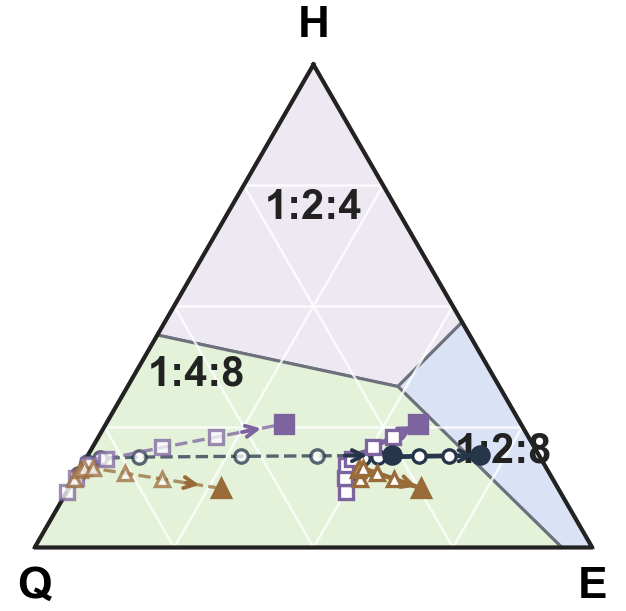
\includegraphics[width=0.40\columnwidth]{k4_n12_prefill_time.png}}\par\smallskip
\subfloat[DP compute energy\label{fig:k4_energy_panel}]{%
  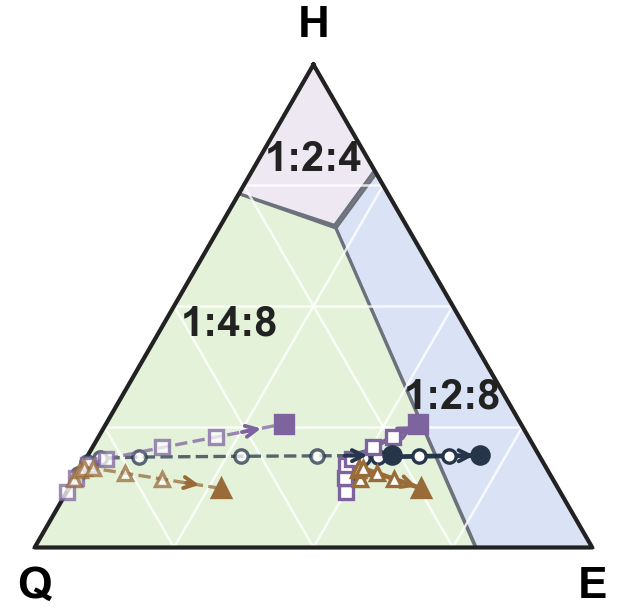
\includegraphics[width=0.40\columnwidth]{k4_n12_prefill_energy.png}}
\caption{Area-constrained ratio selection and prefill trajectories. Colors identify the ratio with (a) minimum compute latency and (b) minimum DP energy. H/Q/E are BF16/FP8/FP4 FLOP shares. Circles, squares and triangles denote V4-Flash, V4-Pro and V4.1-Flash. Dashed lines use W4A8 experts; solid lines use NVFP4 W4A4 experts. Arrows follow 1K, 4K, 16K, 64K, 256K, 512K and 1M contexts; filled markers denote 1M. Energy uses MXFP4 power for both FP4 encodings. Results are model-derived compute estimates.}
\label{fig:k4_time_prefill}
\label{fig:k4_energy_prefill}
\end{figure}

\begin{table}[!t]
\centering
\caption{Optimal-region fractions with MXFP4 as E. Energy fractions are unchanged by integer core deployment.}
\label{tab:k4_regions}
\begingroup\footnotesize\setlength{\tabcolsep}{2pt}
% BEGIN INLINE TABLE: tables/region_table.tex
% Generated by scripts/reproduce.py.
\begin{tabular*}{\linewidth}{@{\extracolsep{\fill}}lrrr@{}}\toprule
Ratio & Time (cont.) & Time (int.) & DP energy \\\midrule
$1:2:4$ & 27.54\% & 33.15\% & 19.48\% \\
$1:2:6$ & 6.66\% & 7.94\% & 2.84\% \\
$1:2:8$ & 8.24\% & 6.63\% & 14.39\% \\
$1:4:8$ & 57.56\% & 52.28\% & 63.28\% \\
\bottomrule\end{tabular*}
% END INLINE TABLE: tables/region_table.tex
\endgroup
\end{table}

H-heavy workloads favor $1:2:4$, E-heavy workloads favor $1:2:8$, and high Q demand favors $1:4:8$. The intermediate $1:2:6$ ratio wins in part of the H/E mixture with limited Q work. With integer deployment, the four latency-optimal regions occupy 33.15\%, 7.94\%, 6.63\%, and 52.28\% of the simplex; the energy-optimal regions occupy 19.48\%, 2.84\%, 14.39\%, and 63.28\%. These are geometric fractions of the uniform workload simplex, not probabilities of real applications.

The $1:2:6$ latency-optimal region grows from 6.66\% with continuous core allocation to 7.94\% with integer deployment. Its smaller area increment permits 34 cores, two more than $1:2:8$, preserving more H throughput. The latter benefits from its longer E reduction when E demand is sufficiently high. Energy boundaries depend instead on mode power per unit capacity, so latency and energy can favor different ratios at the same workload point. A ratio's value depends on incremental circuit cost and deployment granularity, not merely its position between other ratios.

\subsection{Model Precision Demand and Ratio Selection}
\label{sec:k4_prefill}

Using official DeepSeek configurations, inference code, and technical reports~\cite{deepseekv4,deepseekv4flashsource,deepseekv4prosource,deepseekv41source}, we analyze text-only cold prefill for V4-Flash, V4-Pro, and V4.1-Flash at batch size 1 and contexts from 1K to 1M. The reference mapping assigns native MXFP4 indexer dot products to E, W4A8 routed experts and FP8 projections to Q, and BF16 attention and grouped output projections to H. Following published NVFP4 quantization configurations~\cite{nvidia2026v4flashnvfp4,nvidia2026v4pronvfp4,nvidia2026deepseeknvfp4}, a second mapping moves the three routed-expert GEMMs to NVFP4 W4A4 while leaving other computations unchanged. At a fixed context, this transfers work from Q to E without changing H.

GEMMs contribute $2MNK$ FLOPs; MoE counts only active experts. Attention and indexer work follow causal, window, compression, and top-$k$ constraints. V4.1 additionally includes CED encoder prefill, decoder-cache construction, finite-window replay, and cross-layer index reuse~\cite{deepseekv41source}. H/Q/E account for 97.11\%--99.37\% of counted GEMM FLOPs; the remainder is FP32. Both panels overlay context trajectories for the reference W4A8 and expert-W4A4 mappings, with 21 points per mapping.

\begin{table}[!t]
\centering
\caption{Reference W4A8 prefill endpoints. H/Q/E shares are normalized over useful GEMM FLOPs. Speedup and DP energy reduction $\Delta E$ compare $1:4:8$ against $1:2:4$.}
\label{tab:k4_prefill_points}
\begingroup\footnotesize\setlength{\tabcolsep}{4pt}
% BEGIN INLINE TABLE: tables/prefill_compact_table.tex
% Generated by scripts/reproduce.py.
\begin{tabular*}{\linewidth}{@{\extracolsep{\fill}}llcrr@{}}\toprule
Model & $S$ & $x_H/x_Q/x_E$ (\%) & Speedup & $\Delta E$ (\%) \\\midrule
V4-Flash & 1K & 15.25/84.58/0.17 & 1.274 & 6.77 \\
V4-Flash & 1M & 19.07/26.39/54.55 & 1.138 & 3.93 \\
V4-Pro & 1K & 11.54/88.40/0.06 & 1.335 & 7.49 \\
V4-Pro & 1M & 25.59/42.45/31.96 & 1.098 & 3.75 \\
V4.1-Flash & 1K & 14.08/85.86/0.06 & 1.292 & 7.00 \\
V4.1-Flash & 1M & 12.24/60.49/27.27 & 1.291 & 6.65 \\
\bottomrule\end{tabular*}
% END INLINE TABLE: tables/prefill_compact_table.tex
\endgroup
\end{table}

\textbf{Reference W4A8 workloads benefit from FP8 expansion.} All three models are FP8-dominated at short contexts, and every sampled reference point selects $1:4:8$ for both objectives. V4-Flash's E fraction reaches 54.55\% at 1M, but Q still accounts for 26.39\%. The extra FP8 capacity offsets the loss of deployed FP4 capacity relative to $1:2:8$. A majority FP4 workload fraction is therefore insufficient by itself to change the preferred ratio.

\textbf{Context scaling depends on model structure.} Under the reference mapping, V4-Pro's H fraction rises to 25.59\% at 1M, reducing the $1:4:8$ speedup from 1.335 to 1.098. CED and index reuse produce a different trajectory for V4.1-Flash: Q remains at 60.49\% and H falls to 12.24\% at 1M, retaining a 1.291 speedup and 6.65\% DP-energy reduction (Table~\ref{tab:k4_prefill_points}). The relative growth of high-precision attention, FP8 projections, and FP4 indexing jointly determines expansion benefits.

\textbf{W4A4 experts can shift long-context workloads toward $1:2:8$.} After expert quantization, V4-Flash's E fraction rises from 50.52\% at 1K to 70.26\% at 1M, while Q falls to 10.68\%. Among sampled points and under the current power proxy, the energy optimum switches to $1:2:8$ at 512K, followed by the throughput optimum at 1M. V4-Pro and V4.1-Flash retain Q fractions of 18.46\% and 24.54\% at 1M and still select $1:4:8$. FP4 experts and context growth can jointly change the preferred ratio, but residual FP8 demand makes the transition model-dependent.

\subsection{Scope and Resource-Constrained Applicability}

The reported latency is compute service time under sufficient data supply and sequential precision phases using all cores. It excludes shape utilization, K tails, feedback dependencies, communication, and format conversion. Energy includes only DP activity and applies Qwen-based mode characterization to DeepSeek work. It is neither measured DeepSeek energy nor complete-chip energy. Fixed peripheral area constrains deployment but is not converted into peripheral power.

Equal-bandwidth constraints can change the feasible array shape. For a square $m\times m$ array with approximately linear input size $w(k)=kb$, per-core input bandwidth is $2mkb\nu$. Holding this bandwidth fixed reduces allowable $m$ as $k$ grows, and the per-core peak $2m^2k\nu$ may decrease. Chip-level outcomes also depend on core count and bandwidth allocation; this observation does not imply that every expanded ratio is inferior to the baseline.

A power cap similarly requires separating energy per operation from simultaneous activity. The $1:4:8$ Q mode has the highest per-DP power but lower energy per operation than the baseline; both affect sustainable throughput when active-core count is limited. A complete model also needs idle-core, accumulator-storage, peripheral, and data-supply power. Our regions therefore provide an area-constrained compute baseline. Selection under equal bandwidth or a power cap awaits calibration of these system costs.
% END REVIEW PAIR: 06_workload.tex

% BEGIN REVIEW PAIR: 07_conclusion.tex
\section{Conclusion}
\label{sec:conclusion}

DP-Puzzle separates multi-precision coverage from low-precision capacity expansion. Its baseline shares H/Q/E arithmetic through common decoding, segmented multiplication, hierarchical alignment, and fused output processing. Specialized E and QE components remove unnecessary high-precision resources and support internal K expansion or independent-output N composition. At matched peaks, the evaluated K compositions have lower area and low-precision active power but require wider input supply. N composition improves input reuse while increasing accumulator state and nearby output-port demand.

Under a fixed area budget, ratio selection depends on precision-specific work, deployable core count, and energy per operation; all four ratios have distinct optimal regions. Reference W4A8 prefill demand from three DeepSeek models favors $1:4:8$, while W4A4 routed experts shift long-context V4-Flash toward $1:2:8$. These compute-model results show why precision labels or isolated peaks cannot determine a preferred ratio: circuit costs and execution precision must be evaluated together. Accounting for data supply, accumulator storage, and power caps is the next step toward system-level deployment conclusions.
% END REVIEW PAIR: 07_conclusion.tex


\section*{Content Generated by AI}
OpenAI Codex assisted with EDA scripting, interpretation of source code and microarchitecture, experimental modeling, data analysis, plotting scripts, and manuscript organization, drafting, and translation. The authors are responsible for the adopted scripts, results, and all claims in this paper.

\clearpage
\setcounter{DACreferencepage}{\value{page}}
\ifnum\value{DACreferencepage}>7\relax
  \PackageWarningNoLine{DAC2027}{Main text exceeds six pages}%
\fi
\typeout{DAC2027: References start on page \thepage}
\bibliographystyle{IEEEtran}
\bibliography{references/references}
\end{document}
